%\documentclass{tg}
\documentclass[conference,final]{IEEEtran}

\usepackage{graphicx}
\usepackage{epsfig}
\usepackage{subfigure}
\usepackage[hypertex]{hyperref}
\usepackage{subfigure}  
\usepackage{color}
% \usepackage{draftcopy}

\usepackage[small,it]{caption}

\usepackage{multirow}
\usepackage{ifpdf}

\long\def\comment#1{{ \bf \textcolor{magenta}{\bf #1}}}
\long\def\ccomment#1{{ \bf \textcolor{blue}{\bf #1 (SJ)}}}
\newcommand{\F}[1]{\B{\textcolor{red}{FIXME: #1}}}
\newcommand{\C}{\comment}
\newcommand{\CC}{\ccomment}
\newcommand{\fix}[1]{\textcolor{red}{\bf #1}}

\newcommand{\jha}[0]{}
\newcommand{\hartmut}[0]{}
\newcommand{\yaakoub}[0]{}
\newcommand{\ole}[0]{}

\newcommand{\fixme}[1]{ { \bf{ ***FIXME: #1 }} }
\newcommand{\jhanote}[1]{ {\textcolor{red} { ***Jha: #1 }}}
%\newcommand{\jhanote}[0]{}
\newcommand{\jitter}[1]{{$\sigma(\alpha)$}}

\newif\ifpdf
\ifx\pdfoutput\undefined
  \pdffalse
\else
  \ifnum\pdfoutput=1
    \pdftrue
  \else
    \pdffalse
  \fi
\fi

\ifpdf
\DeclareGraphicsExtensions{.pdf, .jpg}
\else
\DeclareGraphicsExtensions{.eps}
\fi

\begin{document}

\title{\large Application Level Resource Selection for Adaptive
  Scientific Applications with Irregular Runtime Characteristics using
  SAGA}

\author{\authorblockN{Shantenu Jha\authorrefmark{1}\authorrefmark{2},
    Yaakoub El Khamra\authorrefmark{1}, Hartmut
    Kaiser~\authorrefmark{1}, Ole Weidner\authorrefmark{1}}
  \authorblockA{\authorrefmark{1} Center for Computation and
    Technology, Louisiana State University, Baton Rouge, 70803}
  \authorblockA{\authorrefmark{2} Department of Computer Science,
    Louisiana State University, Baton Rouge, 70803} }
\maketitle

 \begin{abstract}
   There exist a large class of applications that have irregular
   execution characteristics and highly variable resource requirements
   which are very difficult to predict in advance.  Not only is the
   development of such applications difficult, but the effective
   deployment of such application remains a challenge.  For example,
   as a consequence of irregular execution characteristics dynamic
   resource requirements are difficult to predict a priori thus
   rendering static resource mapping techniques such as workflows
   ineffective.  This paper discusses the design and development of an
   prototype ensemble Kalman filter application, which has varying
   resource requirements and execution characteristics. Even for
   relatively small input problem sizes at each stage, up to several
   hundred models are generated which require from one to sixteen
   processors to solve efficiently; the distribution of the number of
   jobs and the run time-to-completion for a given processor count
   varies by up to an order of magnitude.  Such hard to predict
   run-time characteristics render static, data-flow independent
   scheduling techniques difficult to use. We demonstrate how the use
   of appropriate programming abstractions like SAGA and Cactus enable
   the effective development of applications with non-trivial
   requirements, e.g., run-time resource selection based upon the
   application specific characteristics.  As proof of concept we
   deploy our application on the TeraGrid and show the effective
   utilization of several heterogeneous resources.
 \end{abstract}

 \begin{keywords}
   eScience Application, Middleware Inter-operation, Distributed
   Infrastructure Deployment, Distributed Application Programming,
   Cactus, Performance, SAGA, Programming Abstractions
 \end{keywords}

\section{Introduction}

A key impediment to accelerated development of Grid applications and
consequently the uptake of Grids is the scarcity of high-level
application programming abstractions that bridge the gap between
existing grid middle-ware and application-level needs.  Application
developers are daunted by the complexity of the vast array of
low-level Grid and distributed computing software APIs that currently
exist; APIs have traditionally been developed using a bottom-up
approach that exposes the broadest possible functionality.  Coding
using these bottom-up APIs requires extremely verbose code to
implement even the simplest of application-level capabilities.  Many
Grid computing projects~\cite{gat, cog, realitygrid} recognized the
need for higher-level programming abstractions to simplify the use of
distributed computing for application developers.  The Simple API for
Grid Applications (SAGA) attempts to consolidate community effort and
make ends meet by employing a top-down approach to distributed
computing software infrastructure.  SAGA is the first comprehensive
attempt to provide a programmatic approach for the development of
applications so as to utilize distributed environments, either by
design or by virtue of deployment.  In addition to simplifying the
programming environment for application developers, SAGA insulates
applications from technological, version changes and other low-level
implementation details that regularly occur in the lower layers of the
software stack.

By definition Grids are characterised as dynamic and heterogeneous
environments.  They are dynamic due to time-dependent resources loads,
availability and access patterns; the aggregation of specialised
resources in different administrative domains is one source of the
heterogeneity.  Most tools to address the dynamical nature of the
grids assume a fixed underlying resource requirement.  There exist
several well known examples of distributed applications which in turn
have multiple 'embarrassingly' distributed jobs (or sub-applications)
that are either typically uncoupled or the coupling is between the
master and client application.  Things get significantly more
complicated when there is horizontal coupling between the distributed
jobs, say for example, a global exchange or synchronization point.
Most applications and support-tools for distributed applications
assume that the individual ``jobs'' during the course of their run
life-time will display a well-defined, static execution
characteristics.  However there are class of applications for which
the individual job run time characteristics are inherently difficult
to predict and plan for.  In addition to the class of applications we
investigate here -- Kalman filters~\cite{DataAssim, KalmanPaper},
there are ``first principles'' Grid applications such as
GridSAT~\cite{gridsat03} and applications which based upon resource
aware ``learning'' algorithms~\cite{ majority_voting}, for which it is
both difficult to estimate precisely the resource requirements while
explicitly needing to marshal the distributed resources . For these
applications the resource requirement is dynamic and unpredictable;
interestingly, the resource requirements and utilization might
possibly be dependent upon both the execution trajectory and
underlying infrastructure. Such applications are hard to develop and
deploy, but surprisingly, they have traditionally not received the
same level of infrastructural support for the development. It is
difficult to define a scheduling strategy that will be effective
throughout the execution of a complete applications; hence static
resource mapping is not an option.  It can be argued that the logic
for adapting to resource requirement changes from within the
application are best addressed at the application level.

% -- a specific example of which is the ``Black Oil'' (discussed in
% detailed in section 3) --an important application in petroleum
% engineering,


There has been impressive work in the area of application-level
scheduling~\cite{apples03}, such as AppLeS. It is important to point
out that the logic is encoded in the agent implemented by the AppLeS
developers and that to for a fixed set of distributed patterns
(Master-Worker and Parameter-Sweep).  However there are a much richer
class of programming patterns that applications can be classified
under and it is imperative to support the wider set. Also as pointed
out in Ref~\cite{apples03} it is not easy to programmatically adapt
the application performance characteristics. The approach using SAGA
we adopt in this paper attempts to be the first to provide a
programmatic ability for a general class of applications from a wide
range of distributed patterns.

% The TeraGrid is a distributed infrastructure consisting of a
% collection of high-end, coupled resources; 

The TeraGrid has definitely provided a massive increase in the
computing power available for scientific applications, but this is due
to the individual parts, and nothing to do with the sum of the parts,
ie not because applications are able to use distributed resources in a
coupled or coordinated manner.  it has had limited success in
engendering novel applications or usage modes.  The future of the
TeraGrid \cite{teragridfuture} is at best uncertain; this is in part
due to its inability to provide the platform for any new distributed
programming paradigm or novel application class, some have argued,
rightly so.  The problem is however not localised to the TeraGrid; it
remains difficult to harness other distributed high-end distributed
infrastructure such as DEISA towards a single application

The aim of this paper is to provide a rare example of a novel approach
of developing (programming) an application that can utilize the
individual resources of the TeraGrid in a coupled and coordination
fashion, and not just a single piece of big-iron.  We have captured
the primary run-time characteristics of an interesting and common
class of applications and implemented a solution to effectively manage
this run-time complexity at the {\it application level}.  Our solution
is perfectly acceptable as a proof-of-concept, and modulo deployment
and resource availability issues, our approach will scale to problem
sizes encountered in the many science and engineering problems with
hard-to-predict run-time characteristics.

% 
% Admittedly, the size of our input problem that we use is small, and
% thus makes it unlikely to solve a problem of any real {\it scientific
%   impact} %to the petroleum and energy industry,
% however, 


% tools and support infrastructure to support and plan for resource
% variability have been developed.

% {\it mention the need for programmatic approach versus a grid
%   meta scheduler such as grid way or GR MS. mention that workflows are
%   good for static workloads. this in a way is a autonomic dynamic
%   application..}

% Grid way and other meta schedulers are designed to be able to account
% for dynamic resource characteristics -- fluctuations in availability,
% performance, load or proximity.


% {\it mention that these techniques are useful for first principles applications}
% {\it will need to reference AppLeS: application level scheduling
%   paper~\cite{apples03}}
%Mention what AppLeS does \& doesn't and why this work is different

% Applications that are designed for dynamic and heterogeneous
% environments require the ability to manage varying levels of
% heterogeneity and dynamical resources. 

The specific application that we investigate -- a prototype
implementation of a ensemble Kalman filter using SAGA and Cactus -- is
a particularly interesting case of 'irregular, hard-to-predict run
time characteristics'.  The model needs to run to completion which is
defined as convergence to within a certain value.  The run time of
each model was unpredictable and uncorrelated with the run-time of
models on running on the same number of processors -- a truly
independent variable.  As at every stage, each model must converge to
within a specified value before the next stage can begin, hence
dynamically load-balancing so as to ensure that all models complete as
close to each other as possible is the desired aim.  The number of
stages that will be required is not determined a priori. In the
general case the number of jobs required varies between stages.
Figure 1 shows a schematic of the irregular and hard to predict run
time characteristics of the simulations.

\noindent The highlights of this paper are:

\noindent {\it Utilize the advantages of proper programming
  abstractions, by integrating SAGA and Cactus and demonstrate the
  usefulness for Grid application development:}
Cactus provides the support and features required to implement
adaptivity e.g., checkpoint, restart and migrate thorns. SAGA provides
the ability to implement these features in a specific distributed
environment, for example, move files from location A to location B,
start a job on resource X from resource Y.  Thus the two programming
abstractions that Cactus and SAGA provide are natural complements of
each other.  As alluded to, we do so by interfacing SAGA with Cactus
and thus are able to draw on the many advantages of using SAGA
function calls from within a Cactus application.  The result is an
application that uses these two important application-level frameworks
and abstractions to create a truly distributed application.  SAGA
provides the capability for the the distributed aspects. SAGA provides
a high-level programming interface to Grid functionality, and thus
presents arguably, for the first time ever, the ability to develop
complete and sophisticated applications using simple Grid function
calls.  This paper demonstrates the utility of SAGA for creating
applications that can perform across dynamic and heterogeneous
infrastructure.  Importantly, although we focus on a prototype of a
specific application -- Kalman filtering -- thanks to the architecture
and abstractions used, similar functionality can be trivially
incorporated in more sophisticated and complex applications.

\noindent {\it The development of an application that is adaptive in
  multiple ways:}
A working definition of adaptive applications can be given as
following: an application that can respond to a change in the run-time
environment and manage internally (ie without external user or control
intervention) the associated change of state and control-flow arising
from the change(s) in the run-time environment.  For some
applications, adaptivity as defined here would be an {\it interesting}
feature to have, ie., arguably of academic interest. As we will show,
for applications that have irregular run-time characteristics,
adaptivity is a {\it critical} feature, ie., a necessity.  For
example, once a model of application (as a job) has been mapped to a
resource, it is likely that the same model will have to be mapped to
another resource before the model reaches the desired convergence.
Thus for such applications , it is difficult to statically
(re-)schedule or manually control the execution of the jobs through
the application life-time.

Adaptivity may arise due to the number of processors required by the
many jobs being a variable, as well as the fact that the number of
stages (ie involving global synchronization and subsequent
distribution) is unknown {\it a priori}. There comes a point when
providing the mechanism (logic and control) to the applications
themselves to respond to these changes becomes more efficient and
reliable than leaving it to a scheduler (or a meta-scheduler for that
matter). We believe that this prototype application is well beyond the
transition point and is a classic example of an adaptive application.

The ability of a Cactus application to migrate to a more appropriate
resources based upon network characteristics was demonstrated in
Ref~\cite{escience07}.  We extend the sophistication of adaptivity to
include: migration to better resource, based upon both compute and
network characteristics, and choosing optimal resources to spawn to
based upon local queue characteristics (as well as compute and network
performance). The correct abstractions and programming approach
enables the simple codification of an application that can determine
best resource to migrate to based upon all of the above.

\noindent {\it Automated Resource Selection at Runtime:} The Batch
Queue Predictor (BQP)~\cite{bqp, bqp_url}, is traditionally used for
determining the status of the queue resources available and static
resource mapping. What is enticing about BQP is that it provides
information that is of importance to the class of applications that we
are interested in, namely, the ability to predict with given
probability which resource and when a job (with a specified number of
processors and estimated run-time) is most likely to finish.  This is
typically harder to predict correctly than which resource a job with
specified characteristics is most likely to run first.  {\it This is
  the first application that we are aware of that uses BQP internally
  within an application to make resource selection decisions
  dynamically (at run-time, as opposed to static queries) and
  automatically (the logic of how to process BQP information is
  embedded in the application).}

\noindent {\it Effective Deployment of a non-trivial coupled resources
  on the TeraGrid:} Our application is able to use multiple TeraGrid
resources.  Based upon presentations by TeraGrid Directors (Catlett
and Skow), the distribution of applications usage modes on the
TeraGrid indicate approximately 10 (ie less than 1\% of all
applications) actually use the resources in any sense of coupled
fashion (either as MPICH-G2 jobs, or explicitly marshalling more than
1 resource during the course of a simulation~\footnote{It is important
  to note that this number has essentially remained frozen for several
  years, indicating the lack of new applications and usage modes. A
  significant fraction uses Gateways (portals) and a large number of
  applications use workflow tools}. Our application is a high-end
scientific application which uses SAGA to provide the ability to
couple resources -- either at the application level (via common
namespace, logical files etc) or at the infrastructure level (ie
middleware distribution specific adaptors enable the same
functionality across different distributions).

The outline of the paper is as follows: In the next section we outline
the scientific motivation and then describe the details of the
components of the application that we have developed to use SAGA and
Cactus.  The next section provides details of the algorithm that the
application uses to spawn itself onto a set of resources.  In Section
III, we discuss the architecture of the application. Section IV
provides a brief description of the heterogeneous Infrastructure
(test-bed) that we use to deploy this application. Finally we present
the data collected by this application and some simple analysis in
Section V.

\section{Application: Description and Motivation} 

\subsection{Motivation: Ensemble Kalman Filters}
% Modern reservoir simulators are in essence computer programs that are
% used to model fluid flow in porous media. Reservoir flow modeling
% exists in the context of of the reservoir management function, a
% process that optimizes the interaction between data and decision
% making during the life cycle of a field.  One of the more popular
% popular models is the model that is used to solve for the
%Ensemble Parallel Kalman filters can be used for solving
%multi-component, multi-phase flow of fluids~\cite{AzizSettari, },
%atmospheric modelling~\cite{yaakoub_reference_add} and a whole other
%range of scientific and engineering
%problems~\cite{yaakoubreferenceadd}.  Typical input to such
%simulations of multi-phase flow in porous geometry consists of the
%initial conditions of both fluids (saturation, temperature, pressure,
%density etc.) as well environmental conditions (porosity,
%permeability, depth etc.)

%To ensure the fidelity of the such simulations for real models, data
%from simulations is validated against experimental data. This process
%is referred to as history matching. In this process, a large number of
%simulations with different parameters or initial data, are run and
%their results fitted against the experimental data. When simulation
%results vary from experimental data, the input parameters are modified
%to bring the model closer to the real experimental data. This process
%is repeated until a consistency criteria is observerd. The fitting
%method can be anything from a genetic algorithm, an ensemble Kalman
%filter or a simulated annealing process.  Each has its merits and
%drawbacks.  One of the best methods to perform such convergence
%criteria is the ensemble Kalman~\cite{needreferencehere} filter
%method, and it requires a hard synchronization point where it gathers
%all the data from all the various models and modifies model parameters
%to get better history matching in the iterations to follow.

% Typical reservoir simulations can vary in size from 100 grid points to
% tens of millions of grid points, and a decent model space can contain
% upwards of hundreds of models each with possibly varying size,
% physical model (i.e equations to solve) and more importantly different
% rock and fluid properties.  

Ensemble Kalman filters (EnKF) are widely used in science and
engineering~\cite{DataAssim, KalmanPaper}. EnKF are recursive filters
that can be used to handle large, noisy data; the data can be the
results and parameters of ensembles of models that are sent through
the Kalman filter to obtain the true state of the data. The variation
in model parameters often has a direct and sizable influence on the
complexity of solving the underlying equations, thus varying the
required runtime of different models (thus the availability of the
results).  Varying parameters sometimes also lead to varying systems
of equations and entirely new scenarios. This obviously increases the
computational size requirements as well as memory requirements.  For
example as a consequence of the variation in size the underlying
matrix might become too large or even effectively doubling the number
of the system of equations, which could more than doubles the memory
required to solve the system of equations.
%Variation in non-linear terms in non-linear
%partial differential equations might also change the method used
%to solve the system of equations, which would vary the runtime as well
%as memory cost.

Hence a mechanism to assign models to available resources based on
their expected time to completion and resource requirement is useful.
Such a mechanism would estimate the time a model will spend in the
queue of a resource, the time it needs to run, and the time required
to migrate the data it requires/produces back and forth, and based on
that attempt to minimize the time required to perform each history
matching iteration.  In fact, with changing resource simulation
requirements (as is the case with models that find themselves lagging
behind the rest of the model pack), a mechanism which can take
advantage of of faster, cheaper or more powerful machines is even more
advantageous ~\cite{escience07}.

\begin{figure}
\begin{center}
\includegraphics*[scale=0.36,]{./figures/3StageKalmanFilter}
\end{center}
\caption{Schematic illustrating the irregular execution or
  hard-to-predict run-time characteristics of a prototype
  implementation of an ensemble kalman filter. The end-to-end
  application consists of several stages; in general at each stage the
  number of models generated varies. In the specific case studied in
  this paper, the size and granularity of the models varied within a
  stage. Consequently for any given stage the resource requirements
  varied from 8 processors to 64 processors.  The run time of each
  model was unpredictable and uncorrelated with the run-time of models
  on running on the same number of processors -- a truly independent
  variable. At every stage, each model must converge to within a
  specified value before the next stage can begin, hence dynamically
  load-balancing so as to ensure that all models complete as close to
  each other as possible is the desired aim.}
\label{fig:irregular_execution}
\end{figure}

\subsection{Application Outline}

The aim of our model application is to show the potential and ease of
use of a SAGA-enabled Cactus framework application. Our application
consists of a exemplary distributed simulation that uses the added
SAGA functionality to dynamically determine its ideal migration target
based on ad-hoc and statistical network characteristics and to migrate
itself in a heterogeneous Grid environment.  Although this a model
application it can be easily adapted to more complex scientific
applications.  Furthermore, our model application can be used as an
autonomous benchmarking agent for Grid resources. In this section we
briefly describe SAGA and the Cactus framework and discuss our
motivation to use SAGA to incorporate high-level Grid functionality
into Cactus.

\subsubsection{SAGA}

The Simple API for Grid Applications (SAGA) is an API standardization
effort within the Open Grid Forum (OGF)~\cite{ogf_web} an
international standards development body concerned primarily with
standards for distributed computing.

The specification and implementations of the SAGA API has been guided
by detailed examination of the requirements expressed by existing and
emerging distributed computing applications in order to find common
themes and motifs that can be reused across more than one use-case.
The main governing design principle for the SAGA API is the 80:20
Rule: "Design an API with 20\% complexity that serves 80\% of the
application use cases".  They are intended to cover the most common
application-level distributed computing programming constructs such as
file transfer, and job management.  In general, SAGA embodies the most
commonly required features derived from a broad survey of the
community and provides the most common grid programming abstractions
that were identified by several use cases.

SAGA provides a simple, POSIX-style API to the most common Grid
functions at a sufficiently high-level of abstraction so as to be able
to be independent of the diverse and dynamic Grid environments.  The
SAGA specification defines interfaces for the most common
Grid-programming functions grouped as a set of functional packages.
Version 1.0~\cite{saga-core} of the specification has been submitted
to the OGF editorial pipeline and is currently under review.  It
defines the following packages:

\begin{itemize}
\item File package - provides methods for accessing local and remote
  filesystems, browsing directories, moving, copying, and deleting
  files, setting access permissions, as well as zero-copy reading and
  writing
\item Replica package - provides methods for replica management such
  as browsing logical filesystems, moving, copying, deleting logical
  entries, adding and removing physical files from a logical file
  entry, and search logical files based on attribute sets.
\item Job package - provides methods for describing, submitting,
  monitoring, and controlling local and remote jobs. Many parts of
  this package were derived from the largely adopted
  DRMAA~\cite{drmaa_url} specification.
\item Stream package - provides methods for authenticated local and
  remote socket connections with hooks to support authorization and
  encryption schemes.
\item RPC package - is an implementation of the GGF GridRPC
  API~\cite{gridrpc_url} definition and provides methods for unified
  remote procedure calls.
\end{itemize}

The two critical aspects of SAGA are its {\it simplicity} of use and the
fact that it is well on the road to becoming a community {\it standard}.
It is important to note, that these two properties are 
provide the added value of using SAGA for Grid application development.
Simplicity arises from being able to limit the scope to only the most
common and important grid-functionality required by applications.
There a major advantages arising from its simplicity and imminent
standardization.  Standardization represents the fact that the
interface is derived from a wide-range of applications using a
collaborative approach and the output of which is endorsed by the
broader community.

The SAGA C++ reference implementation~\cite{saga_web} was incorporated
into the Cactus Code Framework in Ref~\cite{escience07} to provide the
needed Grid programming functionality.  We believe this was an
important step in merging two programming abstractions to achieve an
effect that is greater that sum of the parts.

The SAGA C++ reference implementation is being developed in close
conjunction with the OGF standard.  Advert-service package which will
most-likely be incorporated into a future version of the OGF standard.
The SAGA C++ reference implementation comprise a complete set of local
adaptors, an SQlite3 and PostgreSQL advert-service adaptor, and Globus
pre-WS adaptors for file (GridFTP) and job (GRAM2) packages. We will
go onto show how the application uses these features.

\subsubsection{The Cactus Code~\cite{cactus_web}}

Cactus~\cite{X0} is a framework for high performance scientific
computing designed for scientists and engineers to develop and run
codes for solving complex problems.  Developing code for high
performance parallel machines has many challenges including
scalability, efficiency (for computation, communication and
input/output), portability and flexibility. Frameworks such as Cactus
allow scientists and engineers to develop modules which can then be
used together with modules written by other researchers to solve
complex computational problems. The framework provides tools ranging
from basic computational building blocks to complete toolkits that can
be used to solve complex problems in astrophysics, computational fluid
dynamics or other disciplines.  Tools developed in the Cactus Code
framework run on a wide range of architectures including desktop PC's,
supercomputers and computational Grids. Cactus and its associated
toolkits are publicly available for download from the Cactus Code
website.

From an architectural standpoint, the Cactus Code framework consists
of a central part (the ``flesh") and code modules (``thorns").  The
flesh serves as a module manager, scheduling the routines of the
thorns and passing data between thorns.  Thorns perform tasks ranging
from setting up the computational grid, decomposing the computational
grid for parallel processing, providing boundary and initial
conditions.
%, communication of data from one processor to another,
%solving partial differential equations to input and output and
%visualization streaming. There are code modules that provide
%simulation control tools, such as the HTTPD thorn that sets up a web
%server for the simulation and allows researchers to control a
%simulation or view sample output from a web interface.  Thorns can
%also provide custom developed scientific or engineering applications,
%such as computational fluid dynamics or gravitational physics.
%
%Features of Cactus which make it particularly suited to take advantage
%of a Grid environment include its portability, architecture
%independent checkpoint and restart capabilities, steering interface,
%and a well designed interface in the flesh for providing information
%about grid variables, scheduling, parameters and so on.

%Cactus has been a driving application for many Grid computing
% projects.  An early experiment in 2000 called the Cactus
% Worm~\cite{X1} showed how any Cactus application could be autonomously
% migrated around the resources of the eGrid in Europe simply by adding
% a new thorn which used the Globus MDS, GRAM and GridFTP AP Is to access
% Grid capabilities. A later collaboration with the GRADS project added
% dynamic capabilities for resource selection and contract
% negotiation~\cite{X2}.  These experiences led to the EU GridLab
% project which experimented with Cactus migration as a driving
% scenario~\cite{X3}.

% Cactus was also used for early experiments in metacomputing, showing
% how incorporating adaptive techniques into the Cactus driver layer,
% such as dynamic load balancing, configuration of ghostzones, and use
% of data compression could lead to acceptable scaling for large MPI
% applications across multiple supercomputers. This work was awarded the
% Gordon Bell prize in 2001~\cite{Cactus_GordonBell}.

\subsubsection{Why SAGA and Cactus?} 

Because of the modular structure of Cactus, any functionality provided
by a specific thorn is immediately available to any of the other
thorns in the configuration. For this reason we implemented a set of
new Cactus thorns providing an extensible set of functions allowing
the collection of netperf~\cite{netperf_web} based network performance
metrics. Additionally, the extensible nature of this set of thorns
permits additional metrics for any Cactus based application in the
future.  To integrate SAGA functionality into Cactus, a SAGA thorn was
developed that provides the basic SAGA installation information
(header files, libraries etc.)  to the thorns that require SAGA
capabilities.  SAGA provides different packages with a consistent and
uniform flavor, thus implementing thorns that have different
functionality (performance measurement and migrate thorns) using
different SAGA packages is preferable. Last but not least, using SAGA
and Cactus enables applications to specify and customize the network
performance characteristics that it needs; as we shall see later, the
ability to do so is a very useful feature.

% \CC{need to add stuff about saga providing the ability to support
%   programming models such as grid-superscalar and programming patterns
%   such as task-farm and parameter sweeps; Ole a need to get a proper
%   reference for this!}

\subsubsection{BQP}
BQP: Batch Queue Predictor ~\cite{bqp} is a tool that is available
on a number of TeraGrid resources that allows users to make bound predictions of
how much time a job of a giving size and duration will spend in the queue.
This prediction is given with a degree of confidence (probability)
that the job will start before a certain deadline (i.e. the time in the queue).
This information is vital when submitting jobs to various machines
as the longer a job sits in the queue, the longer the delay for the entire stage.
For our application we use the C-API to BQP, and interface it to a BQP thorn that
retrieves the predicted time in queue for jobs of given sizes and estimated durations.

To better predict ensemble behavior we have collected (using the same
BQP Thorn but in a different configuration) detailed BQP data for four
major teragrid machines. The collected data \yaakoub{Need to put in
  tables and histograms} indicates that there are machines where
confidence factors vary significantly over a given run-time. While the
collected data requires detailed statistical and stochastic analysis,
some useful information can be infered by observation. For example,
the confidence of running a job of size XXX lasting YYY seconds varies
by ZZZ with a deadline that varies from WWW to VVVV.  \yaakoub{Need to
  pick a good example of a large variation, so far cobalt seems good,
  lonestar perhaps....}  Suden jumps in the confidence factor or
expected deadline given a minimum confidence factor can indicate a
favorable or unfavorable machine/queue/job-size/job-duration
combination. Further analysis is required, particularly considering
that the application that is run as a job is a parallel-scalable
application and can be resized to run on more nodes for a smaller
time.

\yaakoub{Shantenu this is what you meant by preventative/predictive}
\jhanote{Yes, this conveys the flavour. I will go through the
data and stick up an example or two of the ``preventive'' example}

% \subsection{Talk about additional 'irregular execution' applications}
% Having determined which M resources to use, the way forward could be
% using a Grid co-allocator such as HARC~\cite{harc_url}; that is,
% having identified the best M resources from a network performance
% perspective, we leave the co-scheduling of these M resources to HARC
% which is an implementation of Paxos (two-phase) Commit Algorithm. We
% will report on the interfacing of HARC with SAGA in the future.

\section{Application Implementation and Control Flow} 

\begin{figure}
\begin{center}
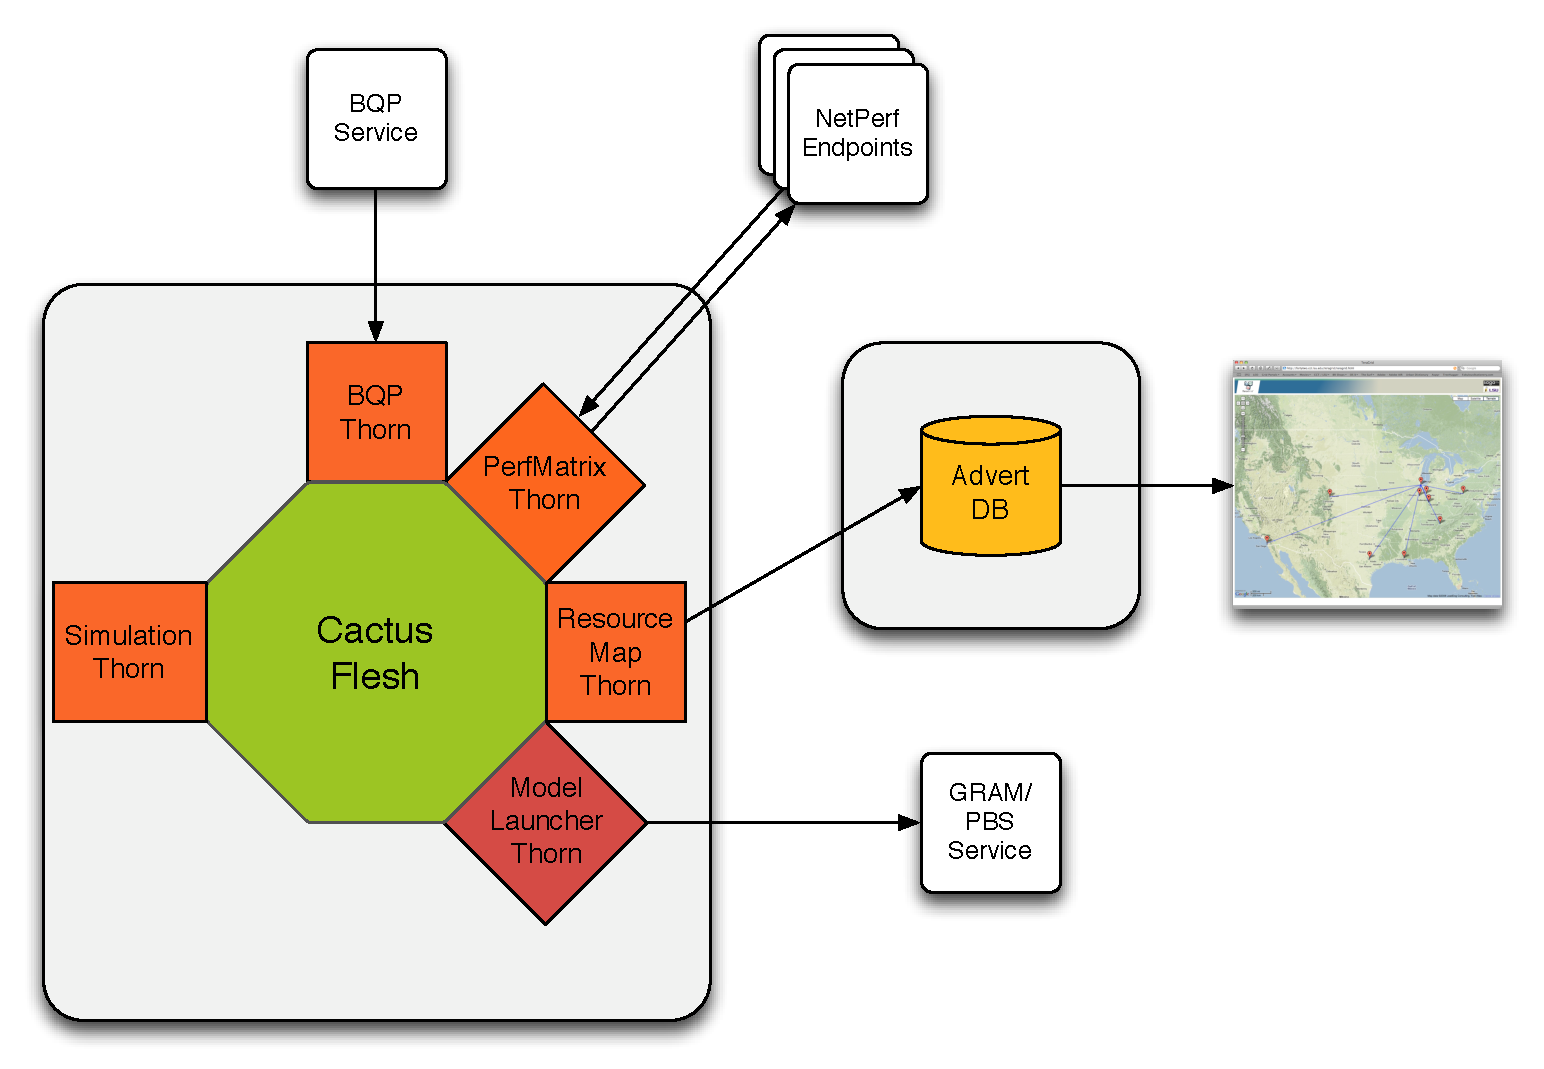
\includegraphics[scale=0.34]{./figures/ApplicationArchitecture}
\end{center}
\caption{The main components of the prototype implementation of Cactus
  based ensemble Kalman filter application. The central orchestrating
  component is the Cactus Flesh; each thorn -- of which there are
  several -- implements a specific, well encapsulated functionality.
  SAGA functionality is provided via a library and is accessed through
  several thorns (such as the Submit thorn).  The thorns are also the
  interface to 'services' such as the Advert service, which in turn
  uses the SAGA API to interface with Google Maps. We believe this is
  an interesting case where an application at run-time is able to
  provide information dynamically to Google Maps. \jhanote{Can we get
    another diagram -- a layered diagram akin to an architecture
    diagram}}
\label{fig:application_architecture}
\end{figure}

%\subsection {Application Architecture} 

\subsection{Simulation Thorn}

This thorn implements the simulation routines for the various models.
Our models are mostly non-linear partial differential equations that
are discretized using finite difference methods and solved with a
Krylov subspace solver using PETSc. ~\cite{PETSc}. For a prototype
implementation we chose a multiphase, multicomponent fluid flow
through porous media simulator and implemented it in the Simulation
thorn in Cactus.
% Is an implementation of the IMPES: implicit pressure explicit saturation 
% method designed to solve two phase flow through porous media problems.
% This thorn requires the thorn {\tt IDBlackOil} to perform the quiescent
% initialization to ensure a balance between gravity and capillary forces 

% The equations we solve are the water and oil mass conservation
% equations with Darcy's law using the IMPES formulation as outlined by
% Aziz and Settari ~\cite{AzizSettari}.  We use a finite difference
% discretization for the implicit pressure equation which we then solve
% by an iterative solver (PETSc) ~\cite{PETSc}.

\subsection{BQP Thorn}
The BQP thorn is a module in Cactus responsible for retrieving the BQP
information using the BQP API. The thorn iterates over all resources
in a given resource list, finds the resource and queue where if
submitted, a reservoir simulation (or model) of a given size and
expected run time, will have a good chance (or high confidence) of
getting through the queue and start running the earliest. Confidence
is in essence the probability that the job will run, and to obtain a
confidence of 1.0, a high queue time is required. For our application,
we found that a confidence of 0.75 works well enough. The information from the BQP thorn is retrieved for all simulations
that need to be run, particularly the time in queue. The time in queue
is added to the time required to run the simulator (which is a
function of the number of nodes and resource used and is retrieved
from regular application benchmarks) and the time required to transfer
data (that is obtained from the PerfMatrix thorn).  That time would be
the estimated time to completion a given models in a given history
matching stage.

\subsection{ResourceMap Thorn}
The ResourceMap thorn maps the various models to available resources.
Each reservoir model has its own parameters that influence the size of
the model and the wall time it will need to finish. \jhanote{In the
  previous line, we need a set of clarifying remarks about how this is
  derived. Does this help?}. The ResourceMap thorn queries the BQP
thorn for the best machine and queue combination that will start the
model earliest at a high enough confidence (i.e above a specified
threshold). This is done by iterating over a list of machines and
their queues, with a constant expected run time and node count and an
increasing ''deadline``, and retrieving the confidence factor of
running before the ''deadline`` from the BQP thorn. If the confidence
is greater than the threshold, the job is submitted. If after
iterating over all machines and queues, we do not get a confidence
factor higher than the specified threshold, the ResourceMap thorn
submits the job to the machine/queue combination that had the highest
confidence factor.

\subsection{Submit Thorn} 
The Submit thorn, as its name suggests, submits a job described by the
ResourceMap thorn to a given resource. A parameter file for the
reservoir simulator and submission script are created at the resource
using SAGA. A SAGA job is then launched that performs the actual
submission (e.g qsub job\_1701.pbs).

\subsection{PerfMatrix} The PerfMatrix thorn takes care of the
intrinsic network performance measurement and persistent storage of
the results. Currently, the implementation uses
netperf~\cite{netperf_web} to measure unidirectional end-to-end
throughput. Netperf is implemented as a simple client-server model
consisting of two executables:
\begin{itemize}
\item{netserver: the measurement endpoint waiting for incoming connections}
\item{netperf: the initiator of a measurement connecting to a netserver endpoint}
\end{itemize}

The PerfMatrix algorithm uses a list of computational resources which
are potential migration targets for the application. After starting
up, the initial application spawns itself onto all available hosts.
\footnote{This approach is different from the original non-centralized
  spawning scheme shown in Fig.~\ref{fig:controlflow} The reason for
  our implementation using centralized spawning is the Globus
  Toolkit's (4.0.5) inability of full credential forwarding.} Once all
jobs have been launched, the original spawning application first
establishes netperf connections with all the spawned applications;
this is followed by the spawned applications establishing netperf
connections amongst each other, following the scheme shown in
Fig.~\ref{fig:controlflow}.  The job spawning, control, and I/O
redirection is done entirely using SAGA's job management package.
Once a netperf process returns a throughput result, the PerfMatrix
thorn uses the SAGA advert-service package to announce the result to a
central PostgreSQL database which is also used as a centralized
logging facility. After all netperf processes have finished and
published their results, the database contains a host-to-host
throughput performance matrix along with a timestamp which is
available to other thorns as well as other applications.

\subsubsection{Advert-service database} SAGA's advert-service package
describes a key-value based hierarchical attribute interface for
storing arbitrary application level information. The currently available adaptor is
capable to map these structures to an relational SQL schema and store
them in local (SQLite) and remote (PostgreSQL) RDBMS. SAGA's advert-service offers a convenient way to simplify the
difficult task of centralized data collection and logging within
distributed applications. The location of all the reservoir
simulations, the start and finish time as well as the paths to the
output files are all stored in the advert-service. The advert-service
also contains the data collected from BQP and from NetPerf.

\subsection{Control Flow}

\begin{figure}
\begin{center}
  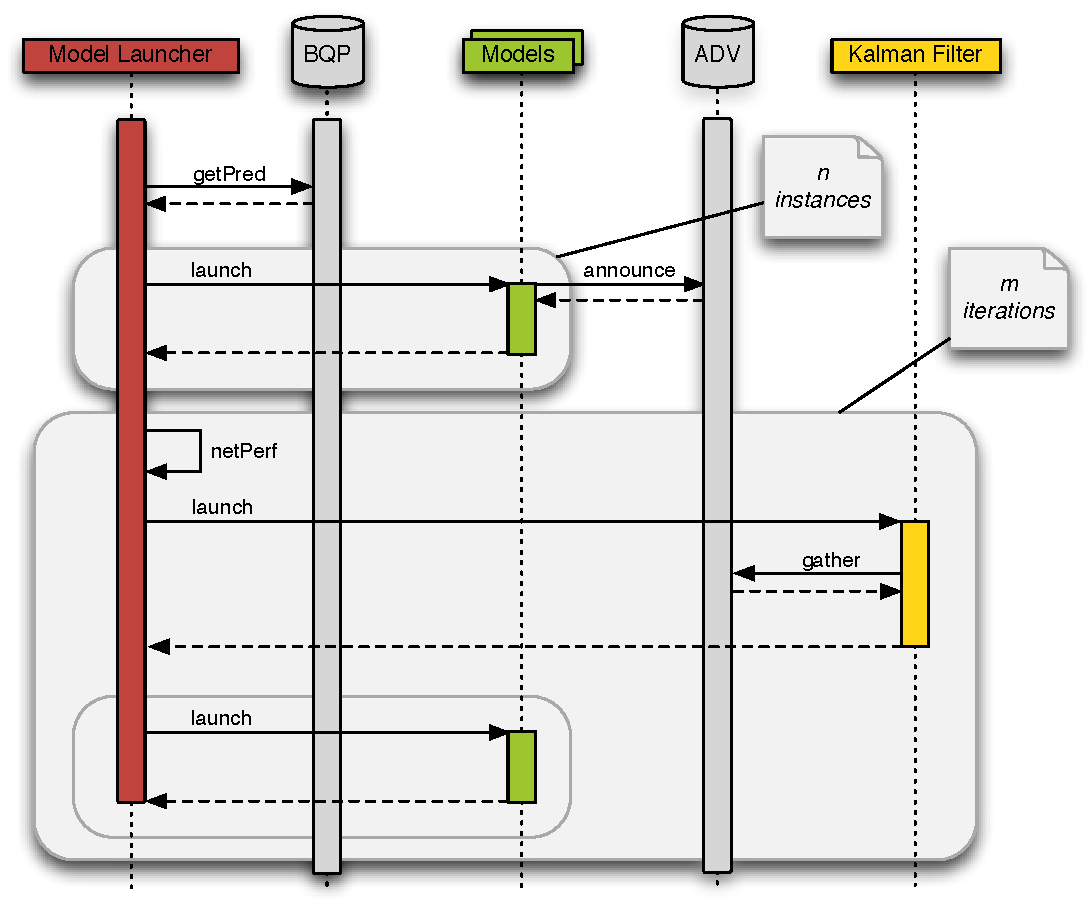
\includegraphics[scale=0.5]{./figures/SequenceDiagram}
\end{center}
\caption{A high-level overview of the control flow for the SAGA-Cactus
  based ensemble Kalman filter application. Models are generated and
  these are mapped to appropriate resources. This is done based upon
  the number of grid points in the model (which in turn determines the
  number of processors and memory) and the projected run-time (which
  is based upon estimated number of iterations). To a first
  approximation the data from BQP is utilized to determine the optimal
  resource -- defined as that resource with the highest chances of
  finishing a job with the prescribed characteristics (number of
  processors, duration) first. Obviously this is just a best effort
  guesstimate, as the actual run-time (number of iterations) is
  difficult to get correct (as it depends upon convergence to a
  value). After all models (n instances) in a given stage have
  finished there is a global synchronization point which in turn is
  the basis for providing models for the next stage (m iterations).}
\label{fig:controlflow}
\end{figure}

The application starts by getting BQP data for a list of candidate
machines, assigns simulations to machines and submits the jobs to the
respective machine scheduler. Once all the simulations are submitted,
the history matching application (in our case a Kalman filter) is
submitted to run. The Kalman filter application is run on the
machine that will run 50\% or more of the entire simulations or the
machine that has the highest bandwidth amongst the machines used for
the simulations.  Once the simulations start, they notify the advert
service of their starting time and location; upon successful
completion, they also notify the advert service of the path of the
files they output.  Meanwhile the history matching application is
notified of the completion of the simulations and modifies the models
used in the reservoir simulation. The modified models are then
submitted again as a second stage and the entire processes is
repeated.

\subsection{Interfacing with Google Maps}

The application level information about the collected BQP and Netperf
data is stored in a central location using the SAGA advert service
facilities. The stored information is usable not only by the
application itself, but is accessible from separate tools allowing to
monitor the application progress. To make this information readily
available to the user we developed a Google Maps~\cite{google_maps}
based user interface presenting the live BQP data for each of the
resources as shown on the map (Figure \ref{fig:gmaps_bqp} shows a
screen shot of this web interface displaying BQP data for the {\tt
  datastar} machine at SDSC). We will add support for displaying the
Netperf based network performance information for each of the network
interconnects as shown on the map as well, as well as extend to show
the physical distribution of sites where jobs are running and the
number of jobs at a site.

Our Google Maps application architecturally consists of two parts.
The client (browser based) side is implemented using Java scripts,
which is the standard way of using the Google Maps API. The server
side (generating the html as requested by the client) is implemented
as a Python based CGI application. We use the SAGA Python API bindings
to access the BQP data stored in the advert service and to generate
the html to display at client side. Whenever the user clicks on one of
the markers or lines in the map we request the corresponding
information from the server by invoking a server side Python CGI
script. The returned html is displayed in the Google Maps info window
pointing to the marker or line the user clicked on.


\begin{figure}
\begin{center}
\includegraphics*[scale=0.34, trim=15mm 33mm 15mm 33mm]{./figures/gmaps_bqp}
\end{center}
\caption{Google maps application showing the live BQP data retrieved
  from the central advert service using the SAGA Python bindings
  (\url{http://fortytwo.cct.lsu.edu/teragrid/teragrid.html}).}
\label{fig:gmaps_bqp}
\end{figure}

\section{Infrastructure Used \& Deployment Details}

\subsection{Infrastructure}
For this trial run we used a pool of TeraGrid machines: Cobalt, SDSC
IA-64 and Queen Bee (QB). The main application starts on Cobalt, runs the
model generator and retrieves the BQP data for all 3 machines.  Since
QB is a new and big machine and the least loaded machine among
the three, it was not surprising when almost all the jobs were
submitted there.  Initially, the application code based the decision
on where to run the Kalman filter on netperf data gathered by the
thorn PerfMatrix. After our initial runs showed that most jobs will be
mapped to QB, the Kalman filter launch code was modified to
take into account where most of the jobs are being run, i.e. running
the Kalman filter on a different machine than 75\% of the jobs would
add more bandwidth cost to the entire stage. Once the jobs are
finished running on QB, the Kalman filter reads in the output
data and modifies the model parameters. These new model parameters
form the basis of the second stage, where the entire process is
repeated as in stage I.

With changing resource requirements during a simulation (as is the
case with adaptive mesh refinement) a mechanism which can take
advantage of faster, cheaper or more powerful machines is even more
advantageous than blind migration. As the primary Cactus simulation
starts, it progresses through the schedule of the routines in the
configuration. One of these routines regularly checks for the time
left for the simulation as well as the the time left for other
simulations, as this information is kept at the advert service. If a
simulation finds itself lagging from the pack, it attempts to migrate
to a resource where it has a better chance of catching up. While most
of this infrastructure is available in the code, it has not been
enabled for these trial runs as it adds more complexity and possible
points of failure.  See:\\
{\tt http://fortytwo.cct.lsu.edu/teragrid/teragrid.html}

\subsection{Deployment}

The deployment of applications across a pool of heterogeneous machines
belonging to different Grids and organizations can be a difficult
task. Different versions and availability of libraries and compilers
makes every single machine a unique environment. Although it is
technically possible to stage-in all required applications and
libraries and even to compile the application sources on the fly using
SAGA, we decided to deploy pre-build binaries on all machines since
this exercise is not part of this work's focus.

SAGA uses a \texttt{autoconf/automake}-based build and installation system
which explicitly tests for available compilers and external library requirements.
Although the SAGA engine itself only depends on the \textit{Boost C++ Libraries} the 
available middleware adaptors may require additional prerequisites which
can range from \textit{PostgreSQL} to the \textit{Globus Toolkit} libraries. The initial attempt
to build and deploy SAGA binaries on TeraGrid resources greatly helped us to realize
that our initial requirements were too progressive and did not work well with 
the rather conservative software deployment strategies in HPC environments.
Based on this experience we started to modify both, the build-system and the
C++ code to allow for more relaxed prerequisites which now comprise:

\begin{itemize}
\item{gcc $\geq$ 3.4 (32 \& 64 bit on i386, x86\_64, and IA64)}
\item{Boost C++ Libraries $\geq$ 1.33}
\item{Globus Toolkit $\geq$ 3.2 (optional)}
\item{PostgreSQL $\geq$ 8.0 (optional)}
\end{itemize}

Currently SAGA is deployed in user space, but should ideally be supported at
the system level due to the limited persistent disk space in the
home directories and to make SAGA transparently available to every user. 
Due to SAGA's latest improvements a system-wide deployment should be a trivial
task which has already been started on the joint LONI/TeraGrid resources.


% Since both, the Cactus framework and SAGA aim to be as
% platform-independent as possible, the deployment process was rather
% straightforward - the only noteworthy problems occurred during the
% initial attempt to build SAGA on LONI's 64bit AIX 5L nodes. \jha{not
%   using LONI! This is TeraGrid}. The problems were mainly caused by the
% IBM's xlC++ compiler's inability to handle C++ partial template
% instantiation, a broken AIX pthread implementation and the absence of
% usable debugging tools. Although the deployment process on AIX was
% very time consuming it eventually led to a vastly improved SAGA build
% system and a more conservative use of C++ template mechanisms which
% ensures the support of other non-standard compilers.

\section{Results and Discussion}

To validate our approach we present our results for a three stage
simulation for a {\it reduced input model} ie. a model with limited
granularity. The model generator produces 200 models of varying size, which are
really models of different requirements -- memory and run-time
duration. These models are mapped to jobs of varying node counts.  For
example, in Stage I of the pipeline the 200 models are mapped so that
173 of them are run on 2 nodes (8 processors), 21 models are mapped to
4 nodes and 6 models are mapped to 8 nodes.  Interestingly the 173
simulations running on say 2 nodes have a wide variation in the
duration that they need to run for (ie determined by a convergence
criterion). For Stage I the fluctuation of 2 nodes jobs was more than
a factor of 2 (min run was 1.68hrs and max run time was 3.5hours). The
fluctuations in run-time are not limited to a set of models for a
given processor count in a single stage; there are significant
fluctuations between the maximum time that models need between
different stages too.  For example the longest running 4 node job in
Stage 1 was 5.99 hours, in stage 2 was 6.18 hours and in Stage 3 was
3.99 hours, which is indicative of the almost factor of 2 difference
in run-time (to convergence) between different stages.

% \jha{yaakoub, is this true for all machines? either way, shouldn't we
%   then just use processors are the basis/unit? Answer: yes and no, I
%   keep the ppn information local to the machine, so it varies. However
%   you are right on QB 1 node=4 procs and you can use that as the unit
%   of measurement},
% (\jha{Yaakoub: Are you sure this isn't a consequence of the max-time
%   specified in the job-submission script?, the x.99 makes me
%   suspicious!! Answer: I cannot dig up the hdf5 files to be sure as
%   these were over-written, but you do raise a valid point})

Simplified as the above may seem there are a few important salient
points that need to be highlighted: The models above were mapped onto
jobs with different resource requirements; here the lower bound and
upper bound are 2 and 8 nodes respectively. However as the granularity
of the input model (problem being studied) is increased, the variation
will get much larger ie upper bound would be of several hundred, if
not thousands of processors 
These in turn will lead to greater variation between individual jobs
for a given processor count in a given Stage, as well as between
different Stages!  The overall fluctuation would be even greater if
the difference between the shortest running job (which might be say a
2 nodes job) and the longest run job (which might be a say a 8 node
job) were considered; even for this reduced model we are looking at
factors of 4 difference if not more.  It is important to note that to
actually impact reservoir simulations, we would have to scale up
details and thus size of our input model by factors of 10 or more.
this would lead to much more complex.%; the shit will hit the fan buddy!
This is proof-of-concept, {\it toy problem} yet took greater than
20,000 CPU hours; any {\it real problem} would require several orders
of magnitude greater resources

% (\jha{yaakoub: check! Anser: yes, we want to run on hundreds of
%   processors per job and the jobs that take a factor of 2 longer may
%   well run into thousands range}).
% (\jha{yaakoub: are these fair estimates? Answer: yes, you will run
%   into this quite easily if we are doing a real, industry standard
%   study}.

\section{Future Work and Conclusion}

Developing both applications and tools using SAGA is an effective
mechanism for ensuring inter-operability across different middleware
distributions -- even at the application level -- something that is
arguably missing in current Grid Interoperation
efforts~\cite{gin_paper} Many challenges remain, but the main are,
program environment heterogeneity -- development, deployment and run
time across resources.  With grids there is the additional
complications of cross-administrative or virtual organizations; as our
paper exclusively uses the TeraGrid, which can for all practical
purposes and intent be considered a single virtual organization, we
are not encumbered by any additional burden. These are serious
challenges for all applications even those that would like to utilize
more than one resource in a decoupled fashion (for example parameter
sweep).  However the seriousness of the heterogeneity problem is
highly aggravated when an application needs to utilize resources in a
coupled manner.

The widespread availability of SAGA (and SAGA adaptors) is an
important step towards the creation of distributed applications that
can be universally deployed (i.e.  independent of the details of the
resource's middleware and configuration detail).  Our experience
should serve as useful input to the community -- resource providers
and middleware developers - to support the development and deployment
of SAGA.  We hope to motivate  resource providers such as the TeraGrid
(as well as middleware developers) to support the SAGA programming
abstractions and thereby help engender applications, as well as
contribute to the development of SAGA , SAGA adaptors as well as
deploying these SAGA adaptors.

We will in the future compare the performance of the execution of such
applications using a meta-scheduler such as Grid way, which although
possibly quicker for some instances will not be as scalable and
extensible. Motivated by the scalability and general purpose solution
we have discussed in this paper, we will go on to generalise to other
applications that exhibit similar characteristics~\cite{nature99}.

% We created a single set of Globus adaptors and deployed them on
% distinct Grids. Our application successfully utilized these
% adaptors, without any further customization, which goes to show that

%We also discussed how the deployment of this model application across
%two distinct Grids was trivial as it only required the deployment of
%of the appropriate SAGA adaptors.  



% There are many applications that need to use federated
% Grids~\cite{clade06, gin_paper}.  Utilizing SAGA to develop, or at
% least provide Grid-functionality is a useful strategy. Therefore, if
% the development and deployment of applications across federated grids
% is to be facilitated, SAGA adaptor activity -- development and
% deployment, needs to be self-sustaining and thus requires explicit
% support, from both the middleware developers and resource providers.

% The success of e-Science critically depends upon the availability of
% e-Infrastructure.  But the promise of e-Science will be hollow without
% delivery of the applications and application-enabling paradigms and
% technology that can effectively utilize this new infrastructure. We
% believe SAGA is an important first step in this direction.

\section{Acknowledgements}

This work has been made possible thanks to the internal resources of
the Center for Computation \& Technology (CCT) at Louisiana State
University.  Important funding for SAGA specification and development
has been provided by the UK EPSRC grant number GR/D0766171/1.  SJ
acknowledges the e-Science Institute, Edinburgh for supporting the
theme, ``Distributed Programming Abstractions''. We would also like to thank Carola Jesch for assistance with
interfacing our output to google maps. Additionally, we would like to
acknowledge help from the LONI support team and CyberInfrastructure
Develompent group.  Y. El-khamra would like to acknowledge Prof. Chris
White, Prof. Mayank Tyagi and Dr. Xin.

\bibliographystyle{IEEEtran}
\bibliography{saga_tg08}
\end{document}

